\documentclass[conference]{IEEEtran}

% correct bad hyphenation here
\hyphenation{op-tical net-works semi-conduc-tor}
\usepackage{graphicx} 
\usepackage{subfig}
\usepackage{verbatim}
\usepackage{fancyvrb}
\usepackage{algorithm}
\usepackage{algorithmic}
\usepackage{cite}

\begin{document}

\title{General Expert System for Anomaly Detection}

\author{\IEEEauthorblockN{Andrew Butcher, Oussama Elrawas, Ekrem Kocag\"uneli}
\IEEEauthorblockA{Lane Department of Computer Science and Electrical Engineering\\
West Virginia University, Morgantown, WV 26506\\
abutcher@afrolegs.com, orawas@gmail.com, ekocagun@mix.wvu.edu}}

% make the title area
\maketitle


\begin{abstract}
The effort to model and understand knowledge and data has given rise to a large variety of implementations of knowledge level modeling. 
Aimed at achieving various operations such as anomaly detection, classification and planning, among others, knowledge level modeling allows us to derive generalizations concerning data. 
In this paper, we present a toolkit aimed conducting KL modeling. 
This toolkit will be presented at this stage of its implementation to allow for anomaly detection in classification data.
By using this toolkit, we implemented a two-step, likelihood-based anomaly detector and tested it on simulated classification datasets for various different scenarios.
Our model has achieved to perfectly identify the normal and abnormal test instances from the simulated datasets.
\end{abstract}

\IEEEpeerreviewmaketitle

\section{Introduction}

Expert systems have been proposed to solve various problems in many different contexts.
Although these systems were developed separately from each other, all of them share common properties. 
The realization of the properties have led to an exciting idea of \textit{knowledge level modeling} (KL).
Knowledge level modeling aims to find abstract patterns of inference that appear in various expert systems \cite{Menzies97object-orientedpatterns:}.

In fact the idea of KL is not a very new concept.
In 70s and 80s, some applications of high level expert systems have been reported.
Although some research was conducted to make this initial work more common and widely applicable, the current trend of expert system design usually consists of a somewhat trial and error approach \cite{Menzies1996}.

Although trial and error method when combined with expert domain knowledge may yield very successful results, most of these models require quite a lot of planning, design and research prior to implementation.
Therefore, the failure to exploit re-usable abstract domain independent problem solving strategies result in waste of resources.
Previous research has also adressed this issue and reported three benefits of using KL modeling \cite{Menzies97object-orientedpatterns:}:
\begin{itemize}
\item Reuse Benefit:New designs can be bootstratpped from previous designs. 
The new design does not need to be a copy of the previous one and may introduce various new configurations.
However, essential pattern will be reused and be the start point of a new design.
\item Communication Benefit: KL models could be very useful to explain various different expert systems and a novice designer with the knowledge of KL models could easily adapt to a new expert system.
\item Guidance Benefit: By analyzing previous models, designers could get an insight regarding where to direct their focus in the design of a new expert system.
\end{itemize}

The fundamental idea behind KL is that a knowledge base is divided into two parts: 1) Domain specific facts and 2) domain independent problem solving strategies \cite{Menzies1996}.
However, a wide range of current expert system designs are not based on this fundamental idea and are missing the afore mentioned benefits provided by KL modeling.

In this research, we are making an analysis of previous KL models and going further we are proposing a common toolbox that includes common methods or tools to these models.
After our analysis, we will build an expert system that will make use of previous KL models and the necessary methods from the common toolbox of KL models.
The model will be applied to a classification dataset and its simulated subsets, which correspond to a generalized version of part one for a knowledge base, i.e. a general representation for domain specific facts.

By building this model on the principles of KL modeling, we do not only exploit the benefits of KL modeling but we also propose a widely applicable model for a large set of domains.

\section{background}
In this section we will describe and briefly discuss previous work related to the area of knowledge level modelling. As discussed in the introduction, KL modelling is well researched concept and there have been several variations on the theme. KL modelling can be presented in one of two different types of studies and implementations: 

\begin{itemize}
	\item General all encumpassing work on knowledge engineering that attempt to cover and implement a wide range of inference functions. These implementations generally do not target a specific type of data.
	\item Specific work on KL modeling that seek to implement a small subset of functionality. Usually such implementations aim at targeting specific data sets.
\end{itemize}

The more encompassing studies seek to implement extensive KL functionality that is able derive knowledge from most data that is available to their system. such work include the modeling of cognitive processes that is presented in \cite{Clancey1985} by Clancey et. al. In this publication, the authors present flowchart style description to several processes that include:

\begin{itemize}
	\item Diagnosis
	\item Verification
	\item correlation
	\item suitability
	\item classification
	\item Prediction
	\item Repair
	\item Design
	\item Configuration
	\item Planning
	\item Scheduling
\end{itemize}

While implementations to these descriptions are not implemented, it is important to take note of them. Such extensive descriptions represent the tradition of knowledge modeling by way of extensive specification of any knowledge/theory producing process. These processes are briefly explained in following sections. As we will see, our own tool is a is based on his tradition of specification~\cite{riesbeck96}.

Detailing current work regarding this approach to knowledge modeling is currently out of the scope of this paper. However, we will briefly present two papers that lie on either side of the fence of this knowledge modeling equation. 

The first paper \cite{Menzies1996} by Menzies provides a description and a system (HT4) that follows the above tradition and which is done through abduction. Abduction here meaning that rules (or hypotheses) are produced such that, given the final effect/state, we are able to most closely determine our initial effect/state. in other words, we are producing rules that will allow us to produce/ infer old data given our current data. This method is obviously dependent on observing enough data to produce out rules. These rules will ultimately define our knowledge. In a similar manner to the cognitive processes document, this work attempts to apply knowledge modeling to achieve several of the functions mentioned above. Such functions include prediction, classification, explanation, tutoring, planning, monitoring, validation, verification and diagnosis. While not identical to the list of functions mentioned above, it overlaps with regard to most of the functionality. As such, the author presents a general tool for use in KL. Our proposed future implementation will be similar to this, with the main difference being that our method is based on induction.

While this ‎is one side of knowledge modeling, the other side of knowledge modeling forgoes specifying all the above functionality, and instead specifies one rule: remember the past to determine the present \cite{riesbeck96}. This is called Case Based Reasoning (CBR). Argued for by Riesbeck, this method represents knowledge and experience with dealing with that knowledge in the form of case bases that include historical data and actions performed on the data in the past. Current actions are determined by the similarity of our current case/data to previous data. This method is based on the principle that people don't create new decisions based on cognitive analysis, but rather that current actions are based on previous actions conducted in similar situations. 

In the next section we will present a description of the model that we will be using.

%One specific applicatio of knowledge modelling is anomaly detection. Anomaly detection is the process of realizing a change in our current data pattern given knowledge of previous data patterns. This is a very extensive field unto itself, with many different implementations. These implementations can implement anomaly detection using many methods, includign but not restricted to:

%-Classification
%-Clustering
%-Nearest Neighbor
%-Statistics.

%In this section, we will briefly go over a two statistical implementations of anomaly detection. 





\subsection{Library and Toolbox For Design Patterns}
\label{section:library}
KL patterns appear in many different expert systems.
In that respect the goal of KL modeling can be defined to identify the abstract reusable inference skeletons that appear multiple times in such systems.
A very good example to this concept is the example of Clancey \cite{Clancey1985}, where he reverse engineered 10 expert system tools with various different characteristics and found out that all of them were using the same abstract inference skeleton: Heuristic classification.
Of course Clancey's example is not the only one.
Another KL methodology KADS \cite{Wielinga1992} was reported to have been used in more than 40 knowledge-based systems \cite{Menzies97object-orientedpatterns:}.

Bearing in mind that KL inferece models are used repeatedly in many different expert systems, it is a good idea to collect and store them.
Clancey proposes a library of pre-defined problem solving strategies and a a separate knowledge-base that contains domain specific heuristics \cite{Wielinga1992}.
In this library we can define common problem solving models that underlie all the expert systems.
When the common problem solving strategy is combined with separate domain specific heuristics, then an expert system can easily be built with less effort.
As examples of models in such a library we can name verification, incremental configuration, systematic diagnosis and heuristic classification.

Going further we would also like to mention a toolbox for such a library that is proposed by Menzies\cite{Menzies2009}.
When we take a closer look to the library proposed by Clancey \cite{Wielinga1992} we see that various problem solving models make use of common methods or algorithms.
For instance verification, classification, sampling methods, diagnosis, discretization, median and greedy agglomerative clustering (GAC) are examples to common methods in the toolbox that can be used by various inference skeletons to form multiple expert systems in different settings.
We can in fact group these algorithms in a toolbox that is available to the use of models in the library of Clancey.

So we can think of building an expert system as a three step process:
\begin{enumerate}
\item Choose a model/template best for your case from the library
\item Pick up required methods from toolbox
\item Insert domain specific heuristics
\end{enumerate}

In our study we will follow the above described three steps to build our model that is capable of processing continuous data and detecting anomalies.
Since we are aiming to provide a generic model, we will not have any domain specific heuristics in our work.
Therefore, we will cover only the first two steps while building our model.

\section{Methodology}

\subsection{Datasets}

In this research we make use of the weather-numerics dataset and its subsets.
Weather-numerics is a classification dataset that has both numeric and categorical features.
Although we have tried only one dataset upto this point, in the following draft(s) we will increase the dataset variety in our research.

Despite the fact that we have a single dataset for the time being, we use multiple subsets of this dataset, which are then simulated with the help of GAC simulation engine.
GAC simulation engine is based on the subsets of the weather-numerics dataset. 
However, the simulated datasets do not have any instances in common.
GAC simulated datasets have close characteristics, but they are commpletely unique datasets.
We will talk more about GAC simulation engine in Section \ref{gac-simulation-engine}.
Therefore, at the end of our analysis we end up covering extensive anomaly detection experiments over many dissimilar datasets.

\subsection{Using Train and Test Sets for Anamaly Detection}

In this section we describe our methodology in producing our subsets for anomaly detection.
While describing our methodology of subset generation, we will use the examaple of weather-numerics dataset, which has 2 classes.
However, this can be extended to an n-many class case easily.
Class labels of the two classes in weather-numerics dataset are \textit{``YES''} and \textit{``NO''}.

While generating subsets, we first choose an anomaly class, say class \textit{NO}.
We select all the instances of class \textit{NO} from the dataset and populate it to $30$ instances.
This will be the so called \textit{anomaly-test-set}.
The remaining instances, i.e. \textit{YES} class instances will be used to generate the \textit{training set} and the so called \textit{normality-test-set}.
To generate the training set, we populate the \textit{YES} class instances to $100$ instances.
Of course in the opposite case, we could have chosen the anomaly class as the \textit{YES} class, in which case \textit{anomaly-test-set} would be the populated \textit{YES} class.
Likewise the \textit{training-set} and the \textit{normality-test-set} would be the populated \textit{NO} class to $100$ and $30$ instances respectively.

In the previous paragraph we have described how we can generate the \textit{normality-test-set}, \textit{anomaly-test-set} as well as \textit{training-set} out of weather-numerics dataset.
However, as can be seen the procedure is easy to generate for an n-class case.
In an n-class case, one of the classes at each turn would be selected as the abnormal class to generate \textit{anomaly-test-set} and the rest will be used to generate the \textit{normality-test-set}.
Since weather-numerics is a relatiely small dataset, we used $30$ and $100$ for the test and train sets respectively.
However, some of the datasets already have more densely populated subsets.
In that case, the test as well as training set sizes could be increased, yet our suggestion is to protect the ratio of test set size over train size around 1/3 .

\subsection{Greedy Agglomerative Clustering Simulation Engine}
\label{gac-simulation-engine}
Since the fundamental method in our model will be the greedy agglomerative clustering (GAC), we will first provide some information regarding GAC.
Agglomerative, or bottom up, clustering starts with every individual
data point and greedily combines similar points using a distance metric \cite{Walter}. Our
model uses euclidean distance to pair similar data points. The
clusters formed can then be mapped into a tree structure. A GAC tree
partitions the data such that the leaves in the tree are the original
data points and each interior node is a cluster containing every point
in its subtree. The root thus contains every data point.
When querying the tree we can easily throw away whole subtrees by
comparing our test with the cluster at hand. This speeds up traversal
greatly, allowing for sub-linear query costs.

A complete GAC tree also allows for data simulation.  By mapping a
dataset into a GAC tree structure we can query the leaf nodes in the
tree to produce an arbitrary amount of new nodes which are a variable
distance between a leaf and it's immediate parent.  Data created this
way will always lie close to a parent/child
pair and will thus be similar the original datasets.

\subsection{Experiments}

Depending on which class of weather-numerics we choose as the abnormal class, we have 2 different treatments in our experimentals settings.
In each treatment, we aim our anomaly dedection model to be able to identify both the abnormal and the normal cases.

In the first treatment, where our anomaly class is the \textit{NO} class, we have a training data of $100$ instances.
The trianing set of $100$ instances are all simulated instances from the \textit{YES} class.
For the simulated train set of \textit{YES} class, we have 2 test sets: \textit{Normality-test-set}, \textit{anomaly-test-set}.
Both test sets are of $30$ instances.
We run our model on both test sets.
In this treatment, since our training set has no instances belonging to class \textit{NO}, we expect all $30$ instances of \textit{anomaly-test-set} to be identified as abnormal cases by our model.
Similar to \textit{anomaly-test-set} instances being identified as anomalies, we expect the \textit{normality-test-set} instances to be identified as normal instances.
That is due to the fact that the \textit{normality-test-set} contains instances that belong to \textit{YES} class only and our train set's normality class is also the \textit{YES} class.

In the second treatment, our anomaly class is the \textit{YES} class.
In this treatment, our training set will have $100$ simulated instances, whose class label is \textit{NO}.
The \textit{normality-test-set} for this treatment will be $30$ simulated \textit{NO} class instances whereas the \textit{anomaly-test-set} will consist of $30$ GAC simulated instances, whose class label is \textit{YES}.

\section{Our Model}

Our model processes incoming new data one instance at a time and tries to dedect anomalies as well as normal instances.
For learning what is abnormal and what is normal, the algorithm relies on past data.
For our case, we use 100 instances in training set.
100 instances are generated by the GAC simulator.
While building our model, we will use the three step procedure that was described in Section \ref{section:library}.
In the following subsections we will describe these steps.

\subsection{Select a template from the library}
Since our aim is to find anomalies with this model, we are in fact dealing with a classification problem where we have two classes: Normal and abnormal.
The most suitable template for the type of problem we are tryinig to tackle with is "heuristic classification".

\begin{figure}
\begin{center}
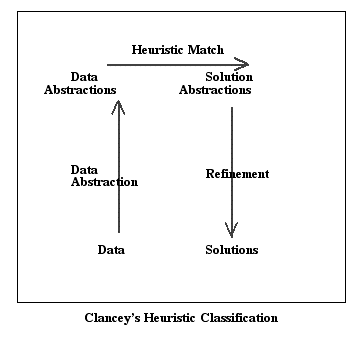
\includegraphics[width=0.5\textwidth]{heuristic_classification.png}
\end{center}
\caption{Heuristic classification takes raw data and applies and abstraction. Then on the data abstraction heuristic match methods are run, which in our case is a likelihood-based two step procedure. Then hypothesis coming from the heuristic match is evaluated and the solution is reached.}\label{fig:heuristic}
\end{figure}

\subsection{Pick up methods from toolbox}
Now we have a basic frame to build our model, but we need to select the appropriate tools to be able to implement this model.
To abstract our data we expect the them to be provided in the form of a two dimensional array in which the rows will correspond to instances and the columns will correspond to features of the instances.
Then the data will be normalized to the interval of 0 to 1 and this will form our abstracted database.
Therefore, we will use a \textbf{\textit{``normalize''}} method from the toolbox first.
Furthermore, since we use GAC tree to simulate our test and training sets, we will need a \textbf{\textit{``GAC''}} method where we also need to calculate the distances between clusters.
Thus, we will pick up a \textbf{\textit{``distance''}} function from the toolbox as well.
We calculate the distance of a single instance to the centroid of clusters in GAC, and centroids are represented by the mean of all the features of all the instances in that cluster.
Therefore, we will also select \textbf{\textit{``mean''}} method of the toolbox.

\begin{figure*}
\renewcommand{\baselinestretch}{1}
\begin{algorithmic} \footnotesize
\STATE $minNumerics \gets minimum(all numeric columns)$
\STATE $maxNumerics \gets maximum(all numeric columns)$
\STATE $minProbNonNumerics \gets minimum(likelihood(all non-numeric columns))$
\STATE $maxProbNonNumerics \gets maximum(likelihood(all non-numeric columns))$
\STATE $testInstance \gets selectOne(test-set)$
\STATE $minNumericsTest \gets minimum(all numeric columns of testInstance)$
\STATE $maxNumericsTest \gets maximum(all numeric columns of testInstance)$
\STATE $test1_{min} \gets isBetween(minNumericsTest,minNumerics,maxNumerics)$
\STATE $test1_{max} \gets isBetween(maxNumericsTest,minNumerics,maxNumerics)$
\IF {$isTrue(test1_{min},test1_{min})$} 
        \STATE $continue$
\ELSE
        \STATE $testInstance \gets anomaly$
\ENDIF 
\STATE minProbNonNumericsTest = minimum(likelihood(all non-numeric columns of testInstance))
\STATE maxProbNonNumericsTest = maximum(likelihood(all non-numeric columns of testInstance))
\STATE $test2_{min} \gets isBetween(minProbNonNumericsTest,minProbNonNumerics,maxProbNonNumerics)$
\STATE $test2_{max} \gets isBetween(maxProbNonNumericsTest,minProbNonNumerics,maxProbNonNumerics)$
\IF {$isTrue(test2_{min},test2_{min})$} 
        \STATE $testInstance \gets normal$
\ELSE
        \STATE $testInstance \gets anomaly$
\ENDIF 
\end{algorithmic}
\caption{Pseudocode for generic anomaly detector. Test-set can be a normal or an anomaly test set. The normality decision can be only made at the end of a succeeding second test, whereas anomaly dedection can be made at any of the two steps.}
\label{figure:trainPseudocode}
\end{figure*}

Once the data is normalized, the heuristic match mechanism will start to work.
Our match mechanism or so called model is a likelihood based model that consists of two rejection/acception steps.
In each rejection/acception step, we decide for a test instance whether to accept it as a normal case or whether to reject it as an abnormal case.
If an instance is rejected in one of the two steps, then we decide that the test instance was an anomaly.

The two rejection/acception steps aim features of different characteristics.
The first step aims numerical features.
In our model we calculate the maximum and minimum values for each numerical feature in training set.
If the test instance's numerical features are above the maximum value or below the minimum value, then this instance is classified as an anomaly and does not make it to the second step.

The second step of the model aims non-numeric features.
In this step, we use a likelihood calculation.
We first calculate the likelihood probabilities of all the instances in the training set.
Then we take the minimum and the maximum probabilities from the training distribution.
The minimum and the maximum probabilities give us an idea of probability range on which the so called normal instances are distributed.
When we calculate the same likelihood probability for the test set, we expect its probability value to fall between the maximum and the minimum probability values of the normal instances.
If the test instance has a probability value outside this range, then we reject it as an anomaly.
On the other hand, if the likelihood probability of the test instance is in this range, then we accept it and call it a normal case.

During training, we produce a frequency table of class counts.  This table contains attribute/range/class values for every instance in the training set which appear as a combination with a count.  For example, [sex, male, pregnant] = 0.  Using this table we calculate the likelihood of an incoming instance by determining the product of each attributes' probability in the instance.

\begin{equation}
product(\frac{frequency [attr, range, "seen"]}{frequency ["seen"]})
\end{equation}

As stated previosly, we assign a probability of 1 to a numeric attribute which is within the minimum/maximum range of that attribute and a probability of 0 to a numeric attribute which isn't within the range.

Remember that we have two tuning mechanisms in that model.
At each step we have minimum and maximum values that decide on whether an instance is to be labeled as an anomaly or not.
At each step, we can play with the minimum and maximum indicators manually.
If we increase the maximum value and/or decrease the minimum value in each step of the model, then we enlarge the normality zone and let more instances be labeled as normal.
However, if we do the opposite, i.e. decrease the maximum and increase the minimum indicator (thereby increasing the constraint to be a normal case) we will be more strict while selecting a normal case and therefore less instances will be labeled as normal.

We now have the template and the required tools to build our expert system.
The third step would be to insert domain specific heuristics into the model.
However, the model does not target any domain for the time being, therefore we will not include this step.

The model whose specifications have been verbally given above is a generic likelihood-based anomaly detector.
For more detail, we provide the pseudocode in Figure \ref{figure:trainPseudocode}:


\begin{figure*}[th!]
\centering
{\scriptsize 
\begin{tabular}{c|c|c|c} 
 \textbf{Training Set} & \textbf{Test Set} & \textbf{Correctly Identified} & \textbf{Detection Percentage}\\ \hline
$100$ \textit{YES} instances & $30$ \textit{NO} instances & $30$ & $100\%$\\
$100$ \textit{YES} instances & $30$ \textit{YES} instances & $30$ & $100\%$\\
\hline\hline
$100$ \textit{NO} instances & $30$ \textit{YES} instances & $30$ & $100\%$\\
$100$ \textit{NO} instances & $30$ \textit{NO} instances & $30$ & $100\%$\\

\end{tabular}}
\caption{In 2 treatments we have 4 different experiments. For each treatment, we try to identify the normal and abnormal cases. In both treatments, both for normalities and the anomalies our model is able to identify them with 100\% accuracy.}
\label{fig:results}
\end{figure*}

\section{Results}

In this section we present the results of our anomaly detector.
The summary of our results are provided in Figure \ref{fig:results}.
As we can see from Figure \ref{fig:results}, our model is able to detect both the normal cases and the abnormal cases with 100\% accuracy.
We have tested our algorithm on simulated datasets under two different treatments.
In each treatment, we aim to identify the anomalies as well as normalities for different classes.
As we can see, we were successful in doing that for the dataset we use in this research.

\section{Conclusion}

In this research we identified a generic procedure as well as a toolkit to aid this generic procedure of generating expert systems.
Furthermore, by following the proposed generic procedure we developed a sample expert system for anomaly detection.
According to our experiments, the anomaly detector was 100\% successful in identifying the abnormal and the normal cases out of simulated datasets.
Therefore, we have seen that the proposed generic method of generating expert systems as well as the sample system works for the simulated datasets in this study.

A further contribution we made in this research is to use GAC simulating engine.
We used GAC simulating engine to generate/simulate similar but unique datasets out of a single dataset with two classes.
We also provide the means to generalize this model to an n-many class case.

\section{Future Work}
In our experiments, the test datasets were of fixed size ($30$ instances in test sets).
However, we accept the test instances one at a time.
Therefore, the model can be easily modified for streaming data.
One additional tweak to the model for streaming data would be to update the training data from time to time.
In other words, the normal classified test instances could be added to the training set and the min-max values can be updated.
We are hoping to code and experiment this case in our next version of this paper.


\bibliographystyle{abbrv}
\bibliography{references}  % sigproc.bib is the name of the Bibliography in this case

\end{document}


